\documentclass[headinclude,footinclude,a4paper,11pt,final]{scrreprt}

%*******************************************************
% La nuova architettura SECOLI - Linee guida
%*******************************************************

% 
% on Ubuntu we need at least the following packages:
%
%   texlive-fonts-recommended, to solve issues related to some pplr9d font not found
%   texlive-fonts-extra for beramono.sty, required by classicthesis-preamble.sty
%
% texlive-publishers is not needed since we include a local copy of classicthesis
%


\usepackage{chngpage}
\usepackage{calc}
\usepackage{fixltx2e}
\usepackage{graphicx}
\usepackage{lettrine}
\usepackage{rcs}
\usepackage{relsize}

\usepackage{classicthesis-preamble}

\usepackage[parts,eulerchapternumbers,pdfspacing,beramono]{classicthesis}
\usepackage{arsclassica}
% ********************************************************************
% arsclassica-settings
% ********************************************************************




% ********************************************************************
% hyperref
% ******************************************************************** 
\newcommand{\mail}[1]{\href{mailto:#1}{\texttt{#1}}}


% ********************************************************************
% makeidx, multicol
% ********************************************************************
\let\orgtheindex\theindex
\let\orgendtheindex\endtheindex
\def\theindex{%
	\def\twocolumn{\begin{multicols}{2}}%
	\def\onecolumn{}%
	\clearpage
	\orgtheindex
}
\def\endtheindex{%
	\end{multicols}%
	\orgendtheindex
}

\makeindex


% ********************************************************************
% listings
% ********************************************************************

\definecolor{lightergray}{gray}{0.99}

\lstset{language=[LaTeX]Tex,
    keywordstyle=\color{RoyalBlue},
    basicstyle=\normalfont\ttfamily,
    commentstyle=\color{Emerald}\ttfamily,
    stringstyle=\rmfamily,
    numbers=none,
    numberstyle=\scriptsize,
    stepnumber=5,
    numbersep=8pt,
    showstringspaces=false,
    breaklines=true,
    frameround=ftff,
    frame=lines,
    backgroundcolor=\color{lightergray}
} 

\lstset{	morekeywords=%
        {RequirePackage,newboolean,DeclareOption,setboolean,%
        ProcessOptions,PackageError,ifthenelse,boolean,%
        chapterNumber,sodef,textls,allcapsspacing,%
        MakeTextLowercase,orgtheindex,endtheindex,%
        @ifpackageloaded,undefined,sfdefault,%
        DeclareRobustCommand,spacedallcaps,%
        microtypesetup,MakeTextUppercase,lowsmallcapsspacing,%
        lowsmallcapsspacing,spacedlowsmallcaps,
        spacedlowsmallcaps,lehead,headmark,color,%
        headfont,partname,thepart,titleformat,part,
        titlerule,chapter,thechapter,thesection,%
        subsection,thesubsection,thesubsubsection,%
        paragraph,theparagraph,descriptionlabel,titlespacing,%
        graffito,lineskiplimit,finalhyphendemerits,%
        colorbox,captionsetup,labelitemi,%
        myincludegraphics,hypersetup,setlength,%
        definecolor,lsstyle,textssc,subsubsection,%
        graffito@setup,includegraphics,ifdefined,%
        myTitle,textcopyright,myName,lstset,lstnewenvironment,%
        setkeys,lst@BeginAlsoWriteFile,contentsname,%
        toc@heading,@ppljLaTeX,z@,check@mathfonts,%
        sf@size,ptctitle,mtctitle,stctitle,lst@intname,%
        @empty,math@fontsfalse,@ppljscTeX,@iwonaTeX,%
        @iwonascLaTeX,@ctTeX,tw@,ct@sc,@ctTeX,f@family,%
        f@shape,ct@sc,ctLaTeX,ctLaTeXe,@twoe,@sctwoe,%
        texorpdfstring,m@th,ctTeX,@mkboth,ProvidesPackage,%
        theindex,PackageInfo,PackageWarningNoLine,%
        mtifont,mtcindent,@iwonaLaTeX,@ppljTeX,@iwonascTeX,%
        rohead,orgendtheindex,@ppljscLaTeX,%
        @ifclassloaded,toc@headingbkORrp,backreftwosep,%
        backrefalt,backreflastsep,areaset,pnumfont,%
        arsincludegraphics,ExecuteOptions,PackageWarning,textcolor,%
        MessageBreak,ars@@includegraphics,ifcld@backref,rofoot,formatchapter,%
        if@twoside},
        commentstyle=\color{Emerald}\ttfamily,%
        frame=lines}

\lstset{basicstyle=\normalfont\ttfamily}
\lstset{flexiblecolumns=true}
\lstset{moredelim={[is][\normalfont\itshape]{/*}{*/}}}
\lstset{basicstyle=\normalfont\ttfamily}
\lstset{flexiblecolumns=false}
\lstset{moredelim={[is][\ttfamily]{!?}{?!}}} 
\lstset{escapeinside={£*}{*£}}
\lstset{firstnumber=last}
\lstset{moredelim={[is][\ttfamily]{!?}{?!}}}

\DeclareRobustCommand*{\pacchetto}[1]{{\normalfont\ttfamily#1}%
\index{Pacchetto!#1@\texttt{#1}}%
\index{#1@\texttt{#1}}}

\DeclareRobustCommand*{\bibtex}{\textsc{Bib}\TeX%
\index{bibtex@\textsc{Bib}\protect\TeX}%
}

\DeclareRobustCommand*{\amseuler}{\protect\AmS{} Euler%
\index{AmS Euler@\protect\AmS~Euler}%
\index{Font!AmS Euler@\protect\AmS~Euler}}

\lstnewenvironment{code}% 
{\setkeys{lst}{columns=fullflexible,keepspaces=true}%
\lstset{basicstyle=\small\ttfamily}%
}{}

\lstset{extendedchars} 
\lstnewenvironment{sidebyside}{% 
    \global\let\lst@intname\@empty 
    \setbox\z@=\hbox\bgroup 
    \setkeys{lst}{columns=fullflexible,% 
    linewidth=0.45\linewidth,keepspaces=true,%
    breaklines=true,% 
    breakindent=0pt,%
    boxpos=t,%
    basicstyle=\small\ttfamily
}% 
    \lst@BeginAlsoWriteFile{\jobname.tmp}% 
}{% 
    \lst@EndWriteFile\egroup 
        \begin{center}% 
            \begin{minipage}{0.45\linewidth}% 
                \hbox to\linewidth{\box\z@\hss} 
            \end{minipage}% 
            \qquad 
            \begin{minipage}{0.45\linewidth}%
            \setkeys{lst}{frame=none}% 
                \leavevmode \catcode`\^^M=5\relax 
                \small\input{\jobname.tmp}% 
            \end{minipage}% 
        \end{center}% 
} 

\newcommand{\omissis}{[\dots\negthinspace]}

\graphicspath{{Graphics/}}

\hyphenation{Robert Bring-hurst DejaVu
Bera Mono Vera Classic-Thesis suite Knuth Zapf}

\newcommand{\meta}[1]{$\langle${\normalfont\itshape#1}$\rangle$}
\lstset{escapeinside={£*}{*£}}


\DeclareRobustCommand*{\miktex}{MiK\TeX%
\index{miktex@MiK\protect\TeX}%
}

\DeclareRobustCommand*{\metafont}{\MF%
\index{METAFONT@\protect\MF}%
}

\DeclareRobustCommand*{\metapost}{\MP%
\index{METAPOST@\protect\MP}%
}

\DeclareRobustCommand*{\texlive}{\TeX{}~Live%
\index{texlive@\protect\TeX{}~Live}%
}


% ********************************************************************
% biblatex
% ******************************************************************** 

%\bibliography{Bibliography}
%
%\renewcommand{\nameyeardelim}{, }
%
%\defbibheading{bibliography}{%
%\cleardoublepage
%\manualmark
%\phantomsection
%\addcontentsline{toc}{chapter}{\tocEntry{\bibname}}
%\chapter*{\bibname\markboth{\spacedlowsmallcaps{\bibname}}
%{\spacedlowsmallcaps{\bibname}}}}     
%
%  \DeclareCiteCommand{\citeyearpar}[\mkbibparens] 
%  {\boolfalse{citetracker}% 
%   \boolfalse{pagetracker}% 
%   \usebibmacro{prenote}} 
%  {\printtext[bibhyperref]{\printfield{year}}} 
%  {\multicitedelim} 
%  {\usebibmacro{postnote}} 
%
%\makeatletter 
%  \DeclareCiteCommand{\citetalias} 
%  {\usebibmacro{prenote}} 
%  {\usebibmacro{citeindex}% 
%   \bibhyperref{\@citealias{\thefield{entrykey}}}} 
%  {\multicitedelim} 
%  {\usebibmacro{postnote}} 
%\makeatother 
%
%\setcounter{biburlnumpenalty}{9000}
%\setcounter{biburlucpenalty}{9000}
%\setcounter{biburllcpenalty}{9000}


% ********************************************************************
% other commands
% ******************************************************************** 

\newcommand{\ita}[1]{% 
  \begin{otherlanguage*}{italian}#1\end{otherlanguage*}}
  
\DeclareRobustCommand*{\pkgname}[1]{{\normalfont\sffamily#1}%
\index{Package!#1@\textsf{#1}}%
\index{#1@\textsf{#1}}}

\DeclareRobustCommand*{\envname}[1]{{\normalfont\ttfamily#1}%
\index{Environment!#1@\texttt{#1}}%
\index{#1@\texttt{#1}}}

\DeclareRobustCommand*{\optname}[1]{{\normalfont\ttfamily#1}%
\index{Option!#1@\texttt{#1}}%
\index{#1@\texttt{#1}}}

\DeclareRobustCommand*{\clsname}[1]{{\normalfont\sffamily#1}%
\index{Class!#1@\textsf{#1}}%
\index{#1@\textsf{#1}}}

\DeclareRobustCommand*{\cmdname}[1]{\mbox{\lstinline!\\#1!}%
\index{#1@\texttt{\hspace*{-1.2ex}\textbackslash#1}}}

\DeclareRobustCommand*{\classicthesis}{Classic\-Thesis}

\DeclareRobustCommand*{\arsclassica}{{\normalfont\sffamily ArsClassica}}

\DeclareRobustCommand*{\miktex}{MiK\TeX%
\index{miktex@MiK\protect\TeX}}

\DeclareRobustCommand*{\texlive}{\TeX{}~Live%
\index{texlive@\protect\TeX{}~Live}}




% roman numerals
\makeatletter
\newcommand*{\rom}[1]{\expandafter\@slowromancap\romannumeral #1@}
\makeatother

% SVN revision number
\RCS$Revision: 1477 $

\hyphenation{con-fi-gu-ra-zio-ne}
\hyphenation{dis-as-ter}
\hyphenation{do-cu-men-to}
\hyphenation{e-qui-val-go-no}
\hyphenation{ga-ran-ti-sca-no}
\hyphenation{i-stan-ze}
\hyphenation{li-vel-lo}
\hyphenation{o-li-sti-co}
\hyphenation{o-pe-ra-ti-va}
\hyphenation{or-a-cle}
\hyphenation{ri-go-re}
\hyphenation{ri-sor-se}
\hyphenation{vi-ce-ver-sa}

\begin{document}

%*******************************************************
% Titlepage
%*******************************************************

\begin{titlepage}
\pdfbookmark{Titlepage}{Titlepage}

\changetext{}{}{}{((\paperwidth  - \textwidth) / 2) - \oddsidemargin - \hoffset - 1in}{}
\null\vfill

\begin{center}
\large
\sffamily
\bigskip
\bigskip
{\Huge\spacedlowsmallcaps{\myTitle} \\
}

\bigskip
\rule{2cm}{0.4pt}
\bigskip
\bigskip

{\LARGE\spacedlowsmallcaps{\mySubTitle} \\
}

\bigskip
    
\vspace{8cm}

\begin{tabular}{cc}
	\parbox{0.3\textwidth}{
\includegraphics[width=2.5cm]{cube-with-magic-ribbons.pdf}}
	&
	\parbox{0.7\textwidth}{{\Large\spacedlowsmallcaps{Fata Informatica}} \\ 
	{\normalsize
	Roberto Reale \\
	Marta Serpietri \\
	\\
	}}
\end{tabular}

\vfill
X Kal.~Sext. \rom{2013}
\end{center}
\end{titlepage}

%*******************************************************
% Abstract
%*******************************************************

\pdfbookmark{Sommario}{Sommario}

\begingroup
\let\clearpage\relax
~
\vfill
\vfill

\chapter*{Sommario}

Alla luce delle nuove sfide cui il portale web SECOLI è chiamato a far fronte, si esaminano criticità e requisiti, tracciando i lineamenti di una proposta progettuale.

\endgroup
\vfill
\thispagestyle{empty}
\setcounter{page}{1}


%*******************************************************
% Chapter: Premesse
%*******************************************************

\chapter{Premesse}

\lettrine{I}{l portale web SECOLI}\graffito{il portale SECOLI} è uno strumento d'avanguardia che l'Amministrazione offre ai cittadini italiani residenti all'estero.

In linea con i contenuti dell'Agenda Digitale italiana ed europea, il portale eroga per via telematica una vasta gamma di servizi, in precedenza fruibili soltanto recandosi di persona in Consolato.  Anche in quei casi in cui la presenza allo sportello sia necessaria, attraverso le pagine del portale è possibile fissare un appuntamento e predisporre in anticipo i dati di interesse (documenti da produrre, percezioni da corrispondere, etc.).

Il\graffito{canale privilegiato con la comunità residente all'estero} portale si presenta come canale privilegiato tra la sede consolare e la comunità residente all'estero:  di importanza primaria, dunque, in termini di visibilità e prestigio dell'Amministrazione.

\bigskip

\lettrine{D}{a un punto di vista} tecnico, individuiamo nella ``missione'' del portale SECOLI tre aree critiche:
\begin{itemize}
\item comunità mondiale di utenti;
\item suddivisione in un \emph{front end} (esposto su rete Internet, rivolto al connazionale) e in un \emph{back end} (esposto su RIPA, accessibile esclusivamente dagli operatori consolari);
\item interazione complessa con altri servizi e piattaforme MAE, in particolare con il \emph{Sistema Integrato Funzioni Consolari} (SIFC).
\end{itemize}

Ad esse corrispondono i seguenti requisiti di progetto:
\begin{itemize}
\item continuità\graffito{continuità del servizio} del servizio e disponibilità del portale 24 ore su 24, 7 giorni su 7.  L'estensione territoriale e sociale dell'utenza non consente l'individuazione di fasce orarie privilegiate, ma, viceversa, un disservizio che interessi le ore notturne a Roma comporterebbe un costo elevato nelle Americhe o in Asia non soltanto in termini operativi, ma anche e soprattutto di immagine;
\item resistenza\graffito{resistenza ai guasti} ai guasti hardware e software (\emph{fault tolerance}) e predisposizione ad un accesso intenso con potenziali picchi;
\item sicurezza\graffito{sicurezza} dei sistemi e dei dati;
\item capacità\graffito{scalabilità} di crescita e di adattamento alle condizioni di carico (\emph{scalability}). Il progetto, dal canto suo, deve contemplare sin dall'inizio spazi di crescita, in forma tale che sia possibile, in ogni momento, intervenire ad incrementare la potenza di calcolo (mediante aggiunta di nuovi nodi fisici o virtuali) senza ledere la normale operatività del portale e senza necessità di ridisegnare l'architettura;
\item interconnessione\graffito{integrazione} ben definita con altre piattaforme;
\item semplicità di gestione.
\end{itemize}

\bigskip

\lettrine{C}{ome ottenere} il rispetto di questi requisiti-cardine?
\begin{itemize}
\item Ripartizione chiara in moduli indipendenti;
\item ridondanza\graffito{ridondanza} e bilanciamento di ogni unità funzionale;
\item punto unico d'accesso, in cui concentrare le misure di prevenzione degli attacchi;
\item adozione di tecnologie e protocolli standard e aperti (art.~68 del \emph{Codice dell'Amministrazione Digitale});
\item virtualizzazione.
\end{itemize}

\bigskip

\lettrine{D}{al punto di vista} della gestione, le condizioni che rendono un portale come SECOLI adeguatamente fruibile dall'utente equivalgono alle più generali premesse su cui riposa la fornitura affidabile, efficace e ininterrotta di un servizio.

Quest'ultima dipende dai seguenti parametri:
\begin{itemize}
\item un\graffito{best practices} buon progetto, che tenga da conto appropriati standard e buone prassi, consolidate nel tempo e confermate dall'esperienza;
\item la stesura di procedure che coprano tutti gli aspetti operativi, dalla normale manutenzione alle condizioni di emergenza e al \emph{disaster recovery}, e di protocolli che assicurino la continuità operativa.  Si noti che parte integrante di questo aspetto è la puntuale e frequente verifica di tutte le procedure di ripristino, incluse naturalmente quelle che coinvolgono le politiche di backup e restore dei dati;
\item un approccio olistico alla sicurezza, parte integrante del quale è l'adozione di formati aperti di interscambio dei dati (si tengano anche presenti le linee guida normative);
\item una gestione che faccia sue le direttive stabilite in sede di progetto nonché durante i successivi momenti di messa a punto e di aggiornamento;
\item una condivisione libera e piena della conoscenza all'interno del gruppo sistemi, dell'intero progetto SECOLI e dell'Am\-mi\-ni\-stra\-zione.
\end{itemize}

\bigskip

\lettrine{Q}{uesti i criteri} che informano le presenti linee guida progettuali.  Lo spirito che ad essi è sotteso dovrà tuttavia costituire la guida privilegiata anche nelle fasi successive, e in ogni momento della vita del progetto. Fermo restando, naturalmente, il riconoscimento pieno di una perfettibilità del disegno iniziale e della necessità che al confronto continuo con la pratica si accompagni un'attività mai interrotta di revisione.


%*******************************************************
% Chapter: Prospettive
%*******************************************************

\chapter{Prospettive}

\section{Cluster e ridondanza}

\lettrine{O}{ve possibile}\graffito{ridondanza a livello applicativo}, sarà da preferirsi una ridondanza realizzata a livello applicativo o di servizio anziché di nodo.  I vantaggi di quest'approccio sono infatti non indifferenti:
\begin{itemize}
\item flessibilità, granularità e controllo maggiori: dal che, a sua volta, segue la possibilità di implementare efficacemente strategie proattive di intervento a fronte di crash;
\item misure di \emph{server consolidation}, ossia di ottimizzazione delle risorse in modo da ridurre il numero complessivo di server impiegati.
\end{itemize}

La ridondanza è assicurata mediante:
\begin{itemize}
\item la coesistenza di istanze multiple dello stesso applicativo, non necessariamente corrispondenti a nodi virtuali o fisici distinti;
\item tecnologie native, specifiche dei singoli applicativi, che garantiscano ove possibile la cooperazione tra le diverse istanze;
\item impiego\graffito{modulo di smistamento} di un \emph{modulo} o \emph{componente di smistamento}, al quale si chiede di instradare le richieste utente verso una tra le molteplici istanze disponibili.  Tale componente provvederà ad assegnare le richieste in base a criteri di bilanciamento del carico, e potrà implementare, ove richiesto, restrizioni di accesso, oltre naturalmente ad assicurare l'alta disponibilità dell'insieme.
\end{itemize}

\bigskip

\lettrine{I}{n particolare}\graffito{Oracle RAC}, si farà riferimento alla tecnologia nativa \emph{Oracle RAC} per implementare la ridondanza e l'alta disponibilità nell'ambito del database.

\section{Hub dati}

\lettrine{L'}{attuale}\graffito{ex ``Replichetta''} database ausiliario ``Replichetta'', rispondendo alla sua vocazione originaria, s'avvia ad assumere nel nuovo quadro strutturale il ruolo di collettore ed accentratore di ogni flusso dati tra SECOLI ed altri servizi MAE, ad eccezione di quelli gestiti dall'\emph{Enterprise Service Bus}.  Si estende e generalizza, dunque, la primitiva funzione di semplice contenitore dei dati SIFC.

Un\graffito{integrazione con EmbAddress} passo in questa direzione è stato già compiuto, peraltro, con l'allacciamento al database EmbAddress.

Opportune misure potranno poi predisporsi per assicurare una tracciabilità dei dati di transito.

\section{Sistema Geografico Consolare}

\lettrine{I}{l Sistema Geografico Consolare}\graffito{database SCE}, o SCE, è un elemento dell'architettura SECOLI vitale tanto per la normale operatività dell'applicativo, quanto per il dialogo con il SIFC.  Con la designazione SCE s'intende, \emph{in primis}, il database contenente l'estensione territoriale delle circoscrizioni consolari, a cui l'applicativo SECOLI fa riferimento per:
\begin{itemize}
\item determinare la sedi di competenza in vari contesti;
\item trattare la codifica numerica del luogo di nascita, di residenza, di matrimonio, e così via, indispensabile per l'interoperabilità con il SIFC.
\end{itemize}

Il \graffito{gateway SCE} database SCE viene fornito dal gruppo Anagrafe, nel corso di aggiornamenti periodici che coinvolgono simultaneamente il portale SECOLI e i server SIFC decentralizzati delle sedi estere, sotto forma di una collezione di file binari \emph{SQLite}; in un formato, dunque, eterogeneo rispetto a quello preferenziale (Oracle), e tale da richiedere l'intervento di un componente software specializzato: il \emph{gateway SCE}.

\section{Database di stand-by}

\lettrine{L'}{applicazione} dei princìpi progettuali che ispirano questo documento, se condotta ad un livello ulteriore, si evolve in modo naturale nel concetto di \emph{database di stand-by}.  Quest'ultimo è una copia funzionalmente identica del database di esercizio (a cui spetterà la qualifica di \emph{primario}), quiescente in condizioni ordinarie, ma pronta a subentrare in ogni momento, e a tutti gli effetti, al primario al verificarsi di eventi traumatici oppure, più semplicemente, durante attività di manutenzione che richiedano un fermo prolungato.

L'alta disponibilità, la protezione dei dati e le capacità di \emph{disaster recovery} risultato estremamente potenziate dalla presenza di un database replicato; non solo, ma quest'ultimo è l'unica misura progettuale che possa mantenere entro limiti accettabili e controllati il \emph{Mean time to recover} (MTTR), ovvero il tempo necessario per il ripristino di una disponibilità operativa anche a fronte di gravi emergenze.

\bigskip

\lettrine{I}{n termini operativi}, la realizzazione di un database replicato deve rispondere ai seguenti requisiti:
\begin{itemize}
\item assicurare un aggiornamento costante e fluido della replica durante la normale operatività del sito principale;
\item disporre di procedure di scambio rapido (\emph{switch}) tra il database primario e quello di stand-by.
\end{itemize}

Considerazioni\graffito{Data Guard} legate al costo delle licenze dovranno intervenire, in sede di valutazione, a guidare nella scelta tra un meccanismo di replica nativo, che faccia uso cioè degli strumenti propri del prodotto Oracle (la tecnologia \emph{Data Guard} è l'unica in grado di mantenere una copia transazionalmente coerente del database primario), e soluzioni per così dire “artigianali”, che dovranno tuttavia essere concepite, se mai, in modo da ridurre al minimo il rischio di inconsistenze.

\bigskip

\lettrine{P}{er quanto riguarda} le risorse hardware necessarie, esse potranno essere agevolmente ricavate dalla dismissione dell'attuale infrastruttura; ovviamente, va previsto, per il sito di stand-by, un carico di lavoro conseguente ad una attività assai limitata nel tempo.

\section{Monitoraggio}

\lettrine{L'}{architettura proposta}\graffito{monitoraggio proattivo} non potrà dirsi completa senza la scelta di uno strumento di monitoraggio che assista lo staff sistemistico nella pronta percezione dei problemi, nella diagnosi e ricerca dell'eziologia e, nella misura del possibile, anche in un intervento attivo.  Ad un apparato del genere si chiederà, in altre parole, di dotarsi di una “intelligenza” che gli consenta di incrementare la proattività del sistemista, ossia la capacità di prevenire ed anticipare i problemi e, più in generale, i bisogni futuri.

Individuiamo i seguenti requisiti come preferenziali:
\begin{itemize}
\item possibilità di attingere ad un vasto patrimonio di moduli aggiuntivi (\emph{plugin});
\item strumenti di amministrazione che consentano uno sguardo olistico sullo stato dell'intera infrastruttura;
\item supporto\graffito{monitoraggio di rete} per il monitoraggio di apparati di rete tramite protocollo SNMP;
\item capacità di operare in una configurazione distribuita.
\end{itemize}

Per sua natura intrinseca, lo strumento di monitoraggio prescelto dovrà attestarsi al di fuori dell'infrastruttura oggetto della sua supervisione, di modo che un fallimento di questa non ne pregiudichi le capacità di notifica e di intervento.


%*******************************************************
% Chapter: Ambienti
%*******************************************************

\chapter{Ambienti}

\section{Esercizio}

\lettrine{V}{a detto}\graffito{resilienza a carichi elevati} che non è possibile, ad oggi, fornire una stima certa del carico a cui sarà sottoposto il portale SECOLI.  Va però anche osservato che l'utenza potenziale coincide con l'intera comunità italiana all'estero, e che picchi elevati di accesso potranno senz'altro verificarsi.

È importante, pertanto, dotarsi di un'infrastruttura che sia facilmente scalabile, ossia tale da permettere l'accrescimento delle sue risorse (aggiunta di ulteriori nodi), se necessario, con il minor sforzo possibile.

Si\graffito{struttura dell'ambiente} propone, pertanto, la seguente articolazione iniziale:
\begin{itemize}
\item due nodi oppure quattro nodi Oracle Database in configurazione RAC, secondo la disponibilità delle licenze, da ripartirsi idealmente su due macchine fisiche distinte;
\item almeno quattro nodi per application server di front end, ripartiti su almeno due macchine fisiche distinte;
\item \emph{idem} per l'application server di back end;
\item web server Apache o Nginx di front end, in cluster;
\item web server Apache o Nginx di back end, in cluster;
\item almeno quattro nodi per il gateway SCE, con due nodi di smistamento in cluster;
\item Enterprise Service Bus;
\item Hub dati.
\end{itemize}

\begin{figure}[ht]
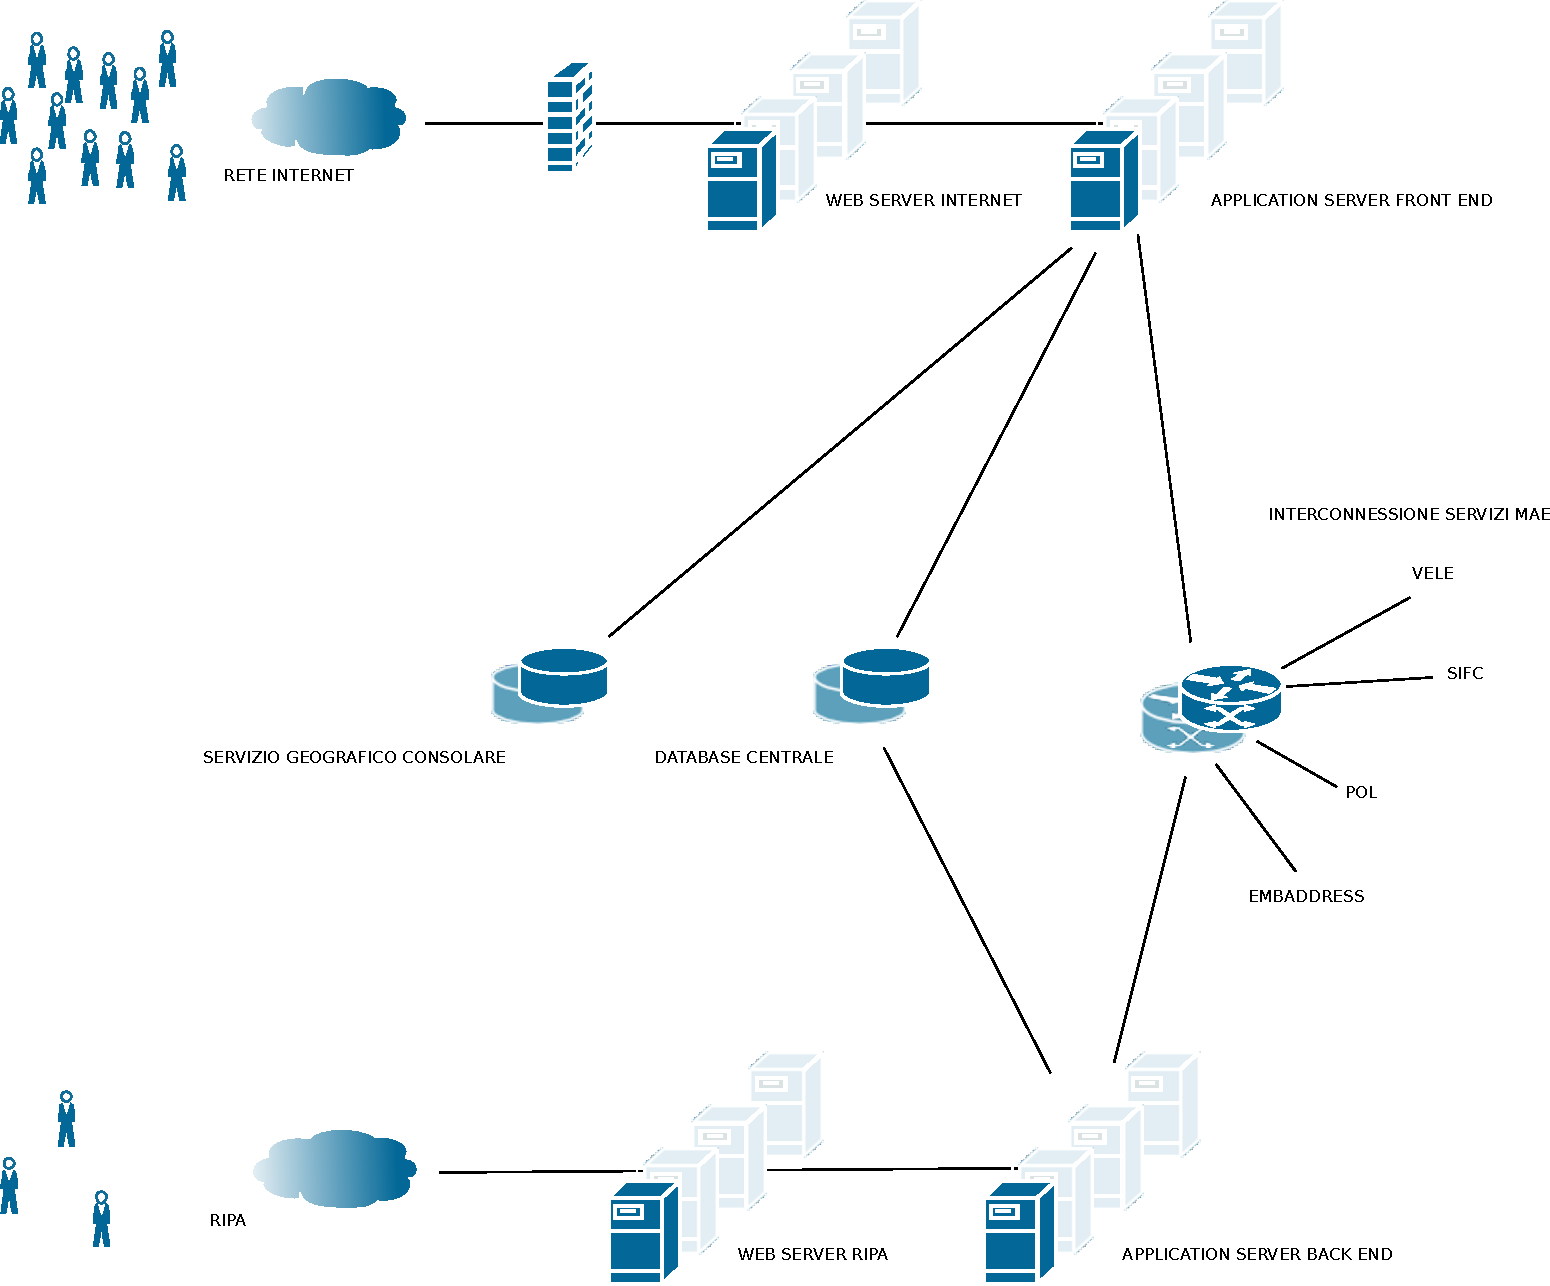
\includegraphics[scale=0.45]{esercizio.pdf}
\bigskip
\caption{Ambiente di esercizio SECOLI}
\bigskip
\bigskip
\end{figure}

\begin{figure}[ht]
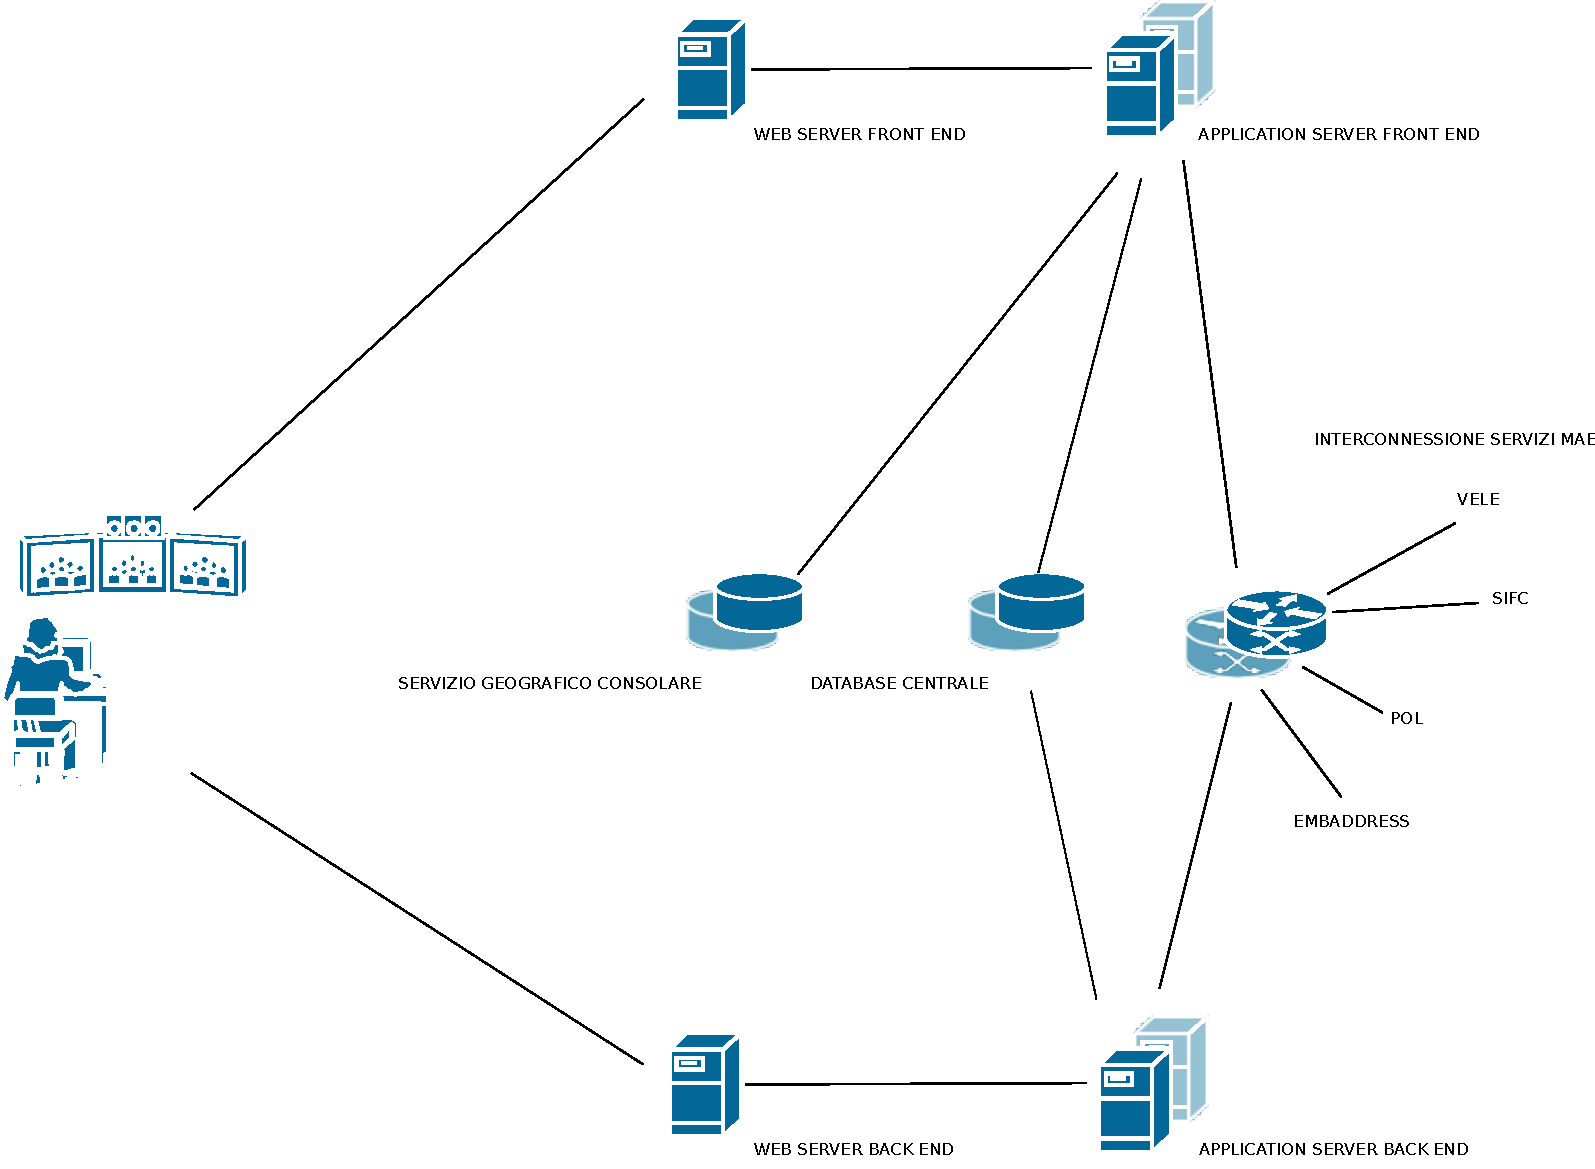
\includegraphics[scale=0.43]{collaudo.pdf}
\bigskip
\caption{Ambiente di collaudo SECOLI}
\bigskip
\bigskip
\end{figure}

\section{Test e collaudo}

\lettrine{L'}{ambiente di collaudo}\graffito{importanza di una buona corrispondenza con l'esercizio} dovrà essere per quanto possibile vicino a quello di esercizio: non in termini di dati, ovviamente, quanto piuttosto di struttura.

Nella pratica corrente si commette sovente l'errore di rinunciare ad un'aderenza piena (il più delle volte per questioni legate ai costi di messa in opera e gestione); noi, tuttavia, insistiamo sulla necessità di mantenere anche nel collaudo in livello almeno minimo di ridondanza, al fine di evitare che problematiche legate intrinsecamente ad un ambiente distribuito non si evidenzino che in esercizio.

Per\graffito{RAC di collaudo} quanto riguarda la base dati, sarà preferibile ricorrere ancora ad una configurazione di tipo RAC (ove lo permettano le licenze).  La complessità aggiuntiva derivante dalla necessità di gestire un secondo ambiente RAC, accanto a quello di esercizio, verrà ampiamente controbilanciata dal vantaggio di un passaggio più fluido e sicuro dal collaudo alla produzione.

\bigskip

\lettrine{S}{i propone}\graffito{struttura dell'ambiente} la struttura che segue:
\begin{itemize}
\item due nodi Oracle database in RAC;
\item due nodi per l'application server di front end;
\item due nodi per l'application server di back end;
\item web server di front end (singola istanza);
\item web server di back end (singola istanza);
\item due nodi per il gateway SCE;
\item singola istanza ESB;
\item Hub dati.
\end{itemize}

I due nodi per il gateway SCE, l'istanza ESB e l'Hub dati potranno essere condivisi con l'ambiente corsi e con quello di sviluppo.

\begin{figure}[ht]
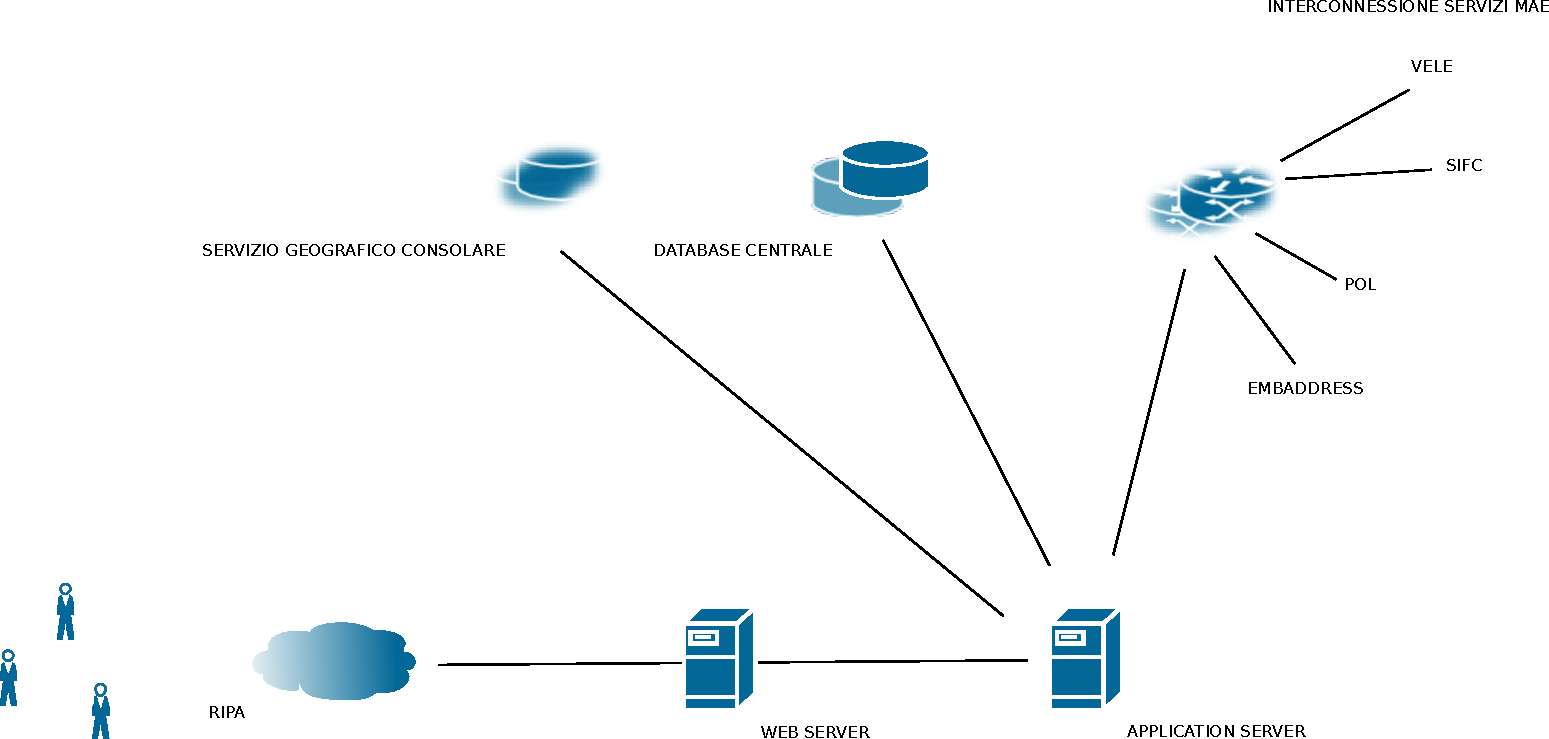
\includegraphics[scale=0.45]{corsi.pdf}
\bigskip
\caption{Ambiente corsi}
\bigskip
\bigskip
\end{figure}

\section{Corsi}

\lettrine{L'}{ambiente corsi}\graffito{specificità dell'ambiente corsi} possiede una sua individualità, situata a metà strada sul continuum che corre dal collaudo all'esercizio.  Esso offre un servizio effettivo ad una comunità di utenti distinti dal gruppo di sviluppo (gli operatori consolari chiamati ad esercitarsi), sicché non viene meno, pur scemandone il rigore, l'imperativo di evitare indisponibilità prolungate.  Va tenuto presente quanto segue:
\begin{itemize}
\item i dati trattati nell'ambiente corsi sono fittizi, ragion per cui non sarà necessario mettere in atto tutto il complesso delle misure di backup tipiche dell'ambiente di esercizio;
\item stante\graffito{infrastruttura non ridondata} il carico di lavoro relativamente modesto, si potrà rinunciare ad implementare un'infrastruttura ridondata;
\item per quel che riguarda l'applicativo vero e proprio, la versione deployata in ambiente corsi dovrà coincidere esattamente con quella in esercizio, salvo speciali esigenze.  Un medesimo automatismo di deploy potrà eventualmente farsi carico di entrambi gli ambienti.
\end{itemize}

\bigskip

\lettrine{S}{i potrà} costruire l'ambiente corsi come segue:
\begin{itemize}
\item database (a singola istanza);
\item application server di front end e web server di front end, ad istanze singole su un nodo condiviso;
\item application server di front end e web server di back end, ad istanze singole su un nodo condiviso;
\item il gateway SCE, l'istanza ESB e l'Hub dati potranno essere condivisi con l'ambiente di collaudo.
\end{itemize}

\section{Sviluppo applicativo \\ sviluppo sistemi}

\lettrine{L'}{ambiente} di sviluppo è, tra tutti, quello che avanza pretese più modeste.  Si predisporrà un pool di macchine destinate ad accogliere l'applicativo (web server, application server) e una macchina ospitante il database.

Sarà\graffito{macchine per lo sviluppo sistemistico} poi indispensabile tenere da parte altre macchine da utilizzare per lo sviluppo sistemistico (ottimizzazione su database, sperimentazione di ambienti, redazione di script) nonché per installazioni SIFC.

\section{Gestione}

\lettrine{P}{iù che di un ambiente}\graffito{strumenti di gestione} vero e proprio, si tratta di una collezione eterogena di macchine deputate a compiti specifici;  tra queste (ma l'elenco non sarà esaustivo) menzioniamo:
\begin{itemize}
\item macchine per il backup: catalogo RMAN per il backup Oracle, server di backup Amanda;
\item collettore dei log;
\item repository del sistema di controllo versione Subversion;
\item file server;
\item gestore di progetto Redmine.
\end{itemize}


%*******************************************************
% About
%*******************************************************

\clearpage
\pdfbookmark{Nota sul documento}{Nota sul documento}

\begingroup
\let\clearpage\relax
~
\vfill
\vfill

\chapter*{Nota sul documento}

A questo documento diede \LaTeX\ veste tipografica.  Il numero di revisione è \RCSRevision.

\endgroup
\vfill
\thispagestyle{empty}

\end{document}
